%%%%%%%%%%%%%%%%%%%%%%%%%%%%%%%%%%%%%%%%%
% University/School Laboratory Report
% LaTeX Template
% Version 3.1 (25/3/14)
%
% This template has been downloaded from:
% http://www.LaTeXTemplates.com
%
% Original author:
% Linux and Unix Users Group at Virginia Tech Wiki 
% (https://vtluug.org/wiki/Example_LaTeX_chem_lab_report)
%
% License:
% CC BY-NC-SA 3.0 (http://creativecommons.org/licenses/by-nc-sa/3.0/)
%
%%%%%%%%%%%%%%%%%%%%%%%%%%%%%%%%%%%%%%%%%

%----------------------------------------------------------------------------------------
%	PACKAGES AND DOCUMENT CONFIGURATIONS
%----------------------------------------------------------------------------------------

\documentclass{article}

%\usepackage[version=3]{mhchem} % Package for chemical equation typesetting
%\usepackage{siunitx} % Provides the \SI{}{} and \si{} command for typesetting SI units
\usepackage{graphicx} % Required for the inclusion of images
\usepackage[section]{placeins}
%\usepackage{natbib} % Required to change bibliography style to APA
%\usepackage{amsmath} % Required for some math elements 

\setlength\parindent{0pt} % Removes all indentation from paragraphs

\renewcommand{\labelenumi}{\alph{enumi}.} % Make numbering in the enumerate environment by letter rather than number (e.g. section 6)

%\usepackage{times} % Uncomment to use the Times New Roman font

%----------------------------------------------------------------------------------------
%	DOCUMENT INFORMATION
%----------------------------------------------------------------------------------------

\title{Gene expression distribution in RNAseq data for mouse and \textit{Eimeria falciformis}} % Title

\author{Totta \textsc{Kasemo}} % Author name

\date{\today} % Date for the report

\begin{document}

\maketitle % Insert the title, author and date

\begin{center}
\begin{tabular}{l r}
%Date Performed: & January 1, 2012 \\ % Date the experiment was performed
%Partners: & James Smith \\ % Partner names
%& Mary Smith \\
%Instructor: & Professor Smith % Instructor/supervisor
\end{tabular}
\end{center}

% If you wish to include an abstract, uncomment the lines below
% \begin{abstract}
% Abstract text
% \end{abstract}

%----------------------------------------------------------------------------------------
%	SECTION 1
%----------------------------------------------------------------------------------------

\section{Objective}

In the differential expression analysis of RNAseq data we assume a negative binomial distribution of transcript abundance. We analyse the distributions in mouse and parasite data respectively. A cutoff is applied to reads mapping per gene in raw data. For instance, a cutoff of ten requires that at least ten reads from \textit{any sample} map to a given gene for the gene to count as expressed. We evaluate the effects of different cutoffs on the distribution. 

%\begin{center}\ce{}\end{center}

%----------------------------------------------------------------------------------------
%	SECTION 2 
%----------------------------------------------------------------------------------------

\section{Results for mouse}

% figure 1
\begin{figure}[h]
\begin{center}
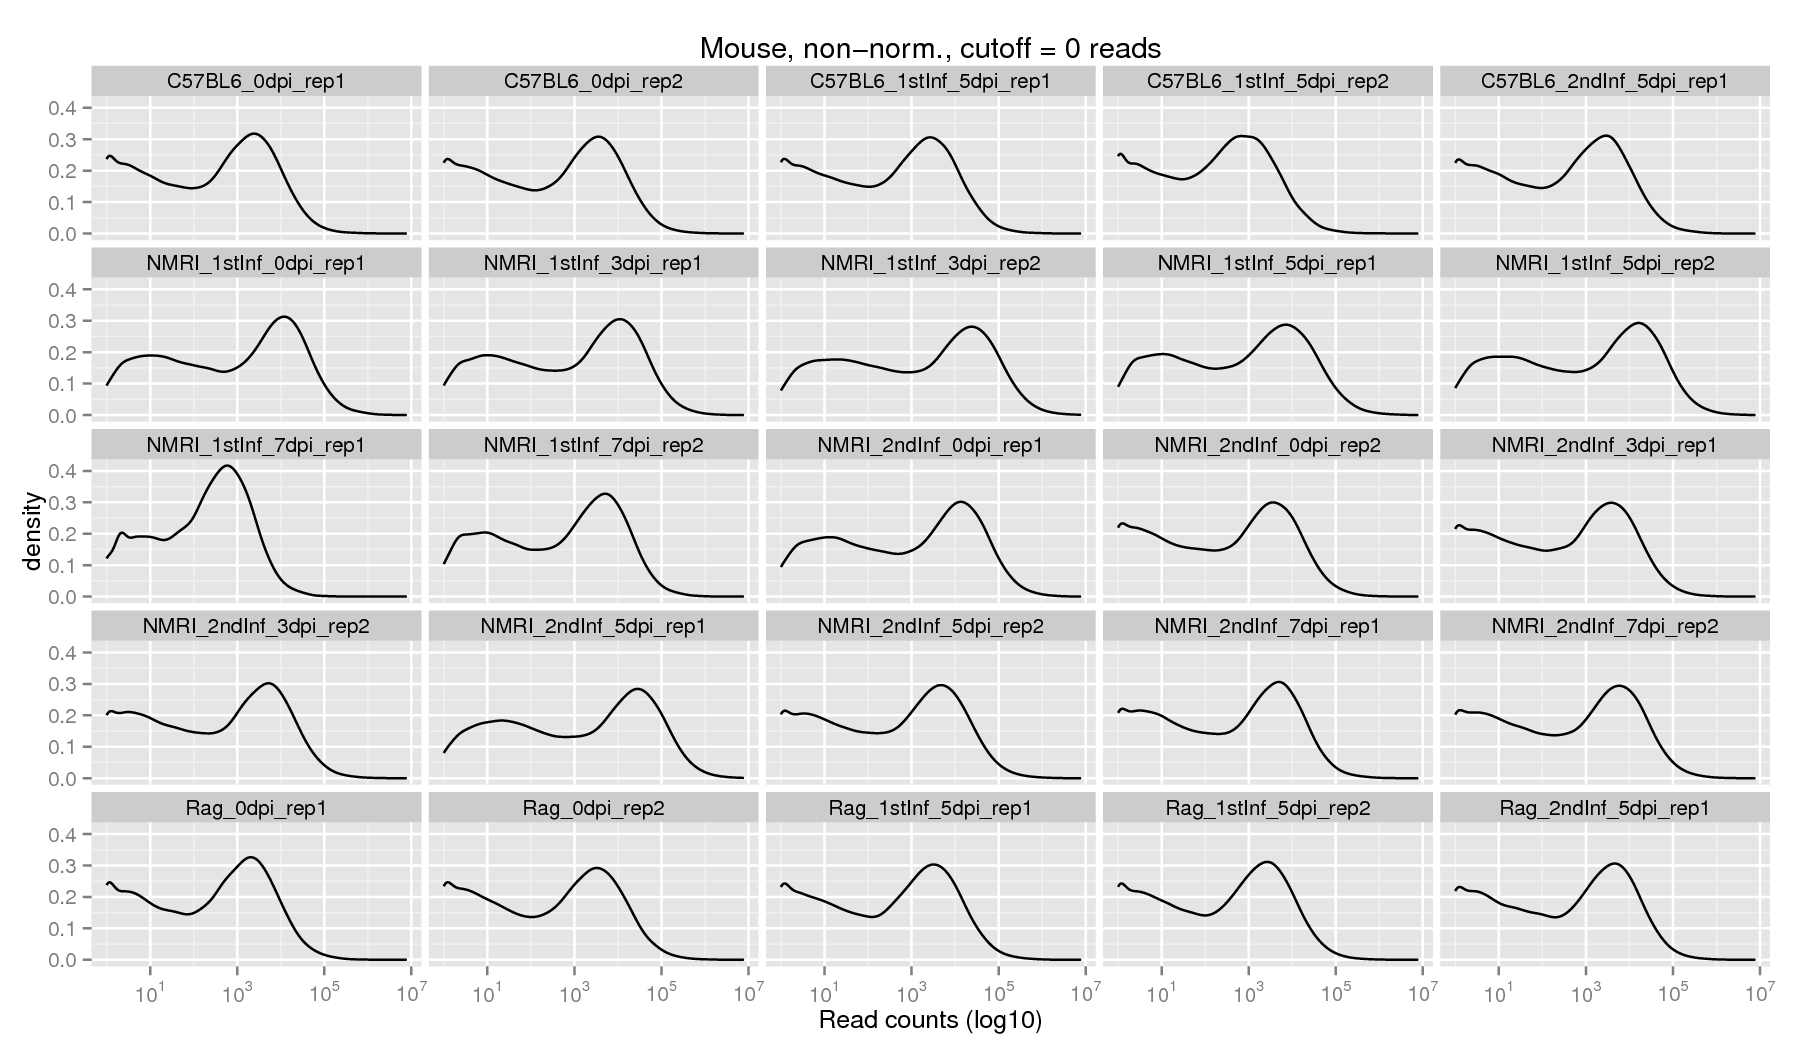
\includegraphics[width=0.8\textwidth]{distributions_mouseNocutoff} % Include the image placeholder.png
\caption{Density distribution of raw transcript counts (log10) for all mouse samples in analysis. All samples share the same bimodal distribution trend by visual inspection. The first density peak occur at $1 - 10^2$ transcripts, \textit{i.e.} transcripts which are detected between 1 and 100 times in that sample. The second density peak occurs in the range of $10^3 - 10^4$.}
\end{center}
\end{figure}

% figure 2
\begin{figure}[h]
\begin{center}
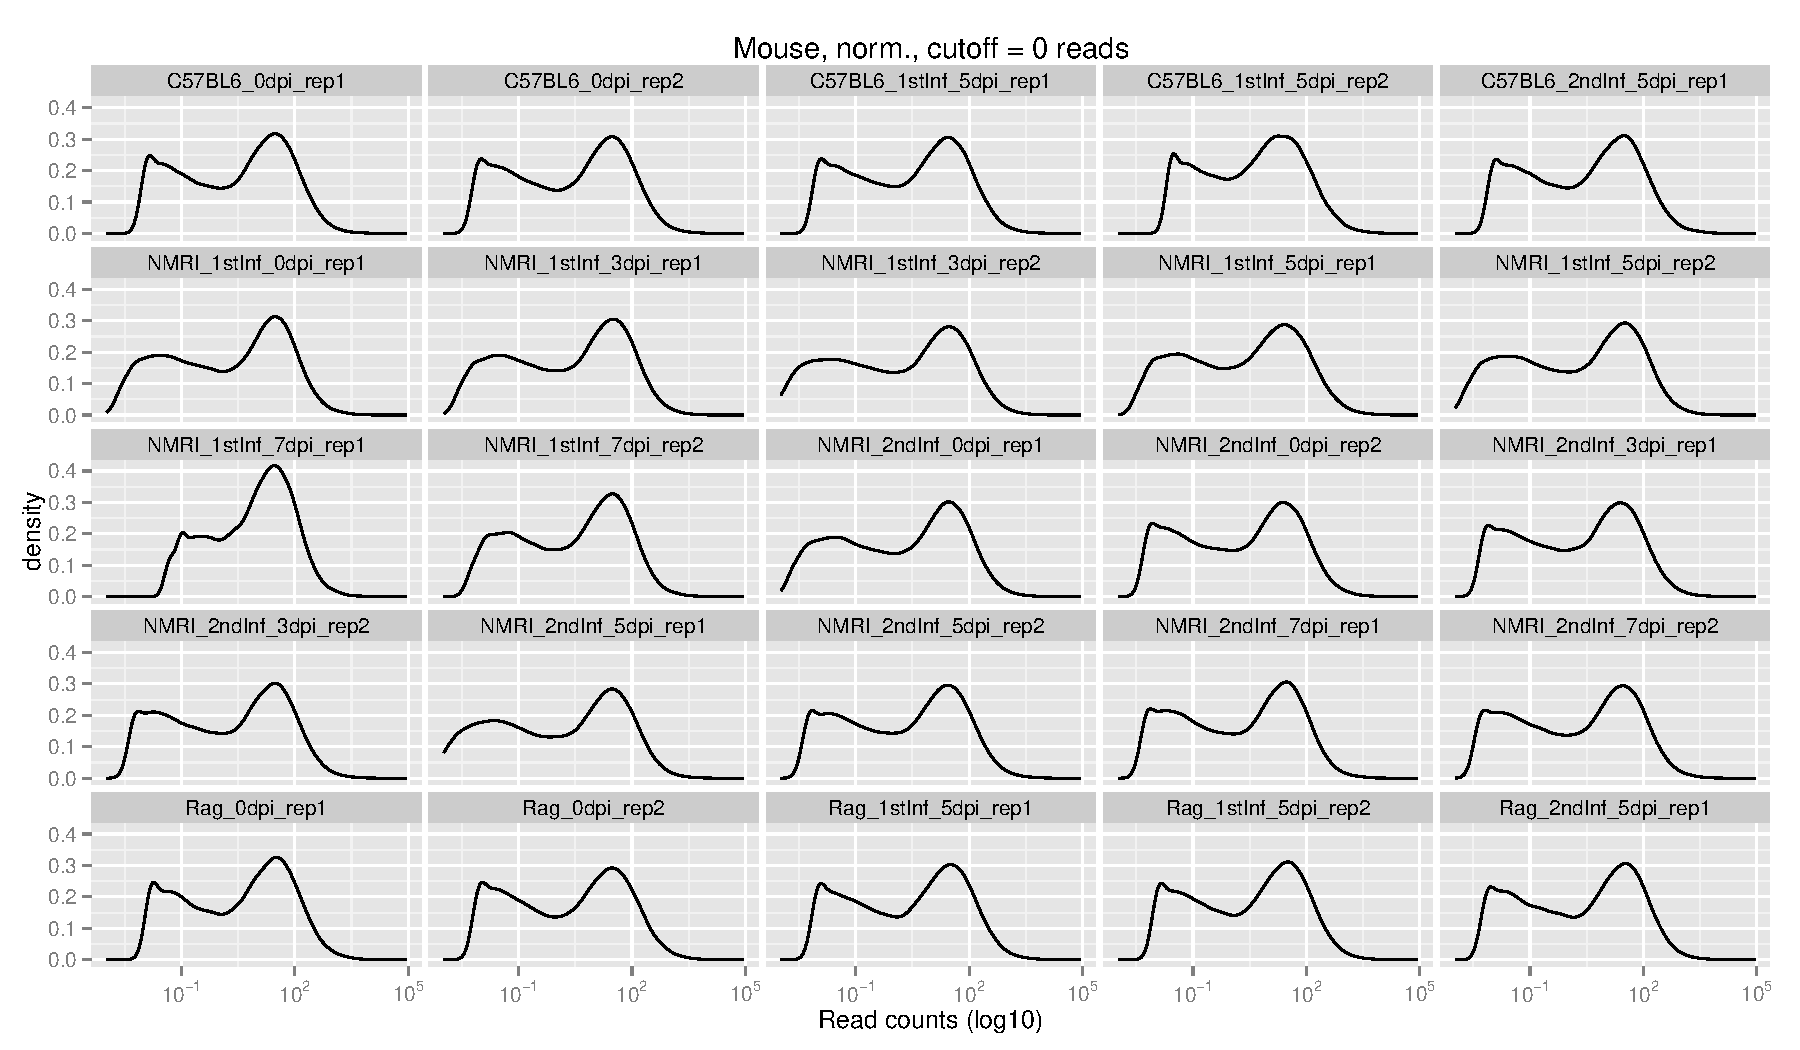
\includegraphics[width=0.8\textwidth]{distributions_normmouseNocutoff} % Include the image placeholder.png
\caption{Density distribution of normalised transcript counts (log10) for all mouse samples. All samples share the same bimodal distribution trend by visual inspection. The first density peak occurs at $<1$ transcripts, and in most samples it is more distinct than in the non-normalised data in Figure 1. For this normalised data, the second density peak occurs at roughly the same count value in all samples, close to $10^2$ transcripts.}
\end{center}
\end{figure}

% figure 3
\begin{figure}[h]
\begin{center}
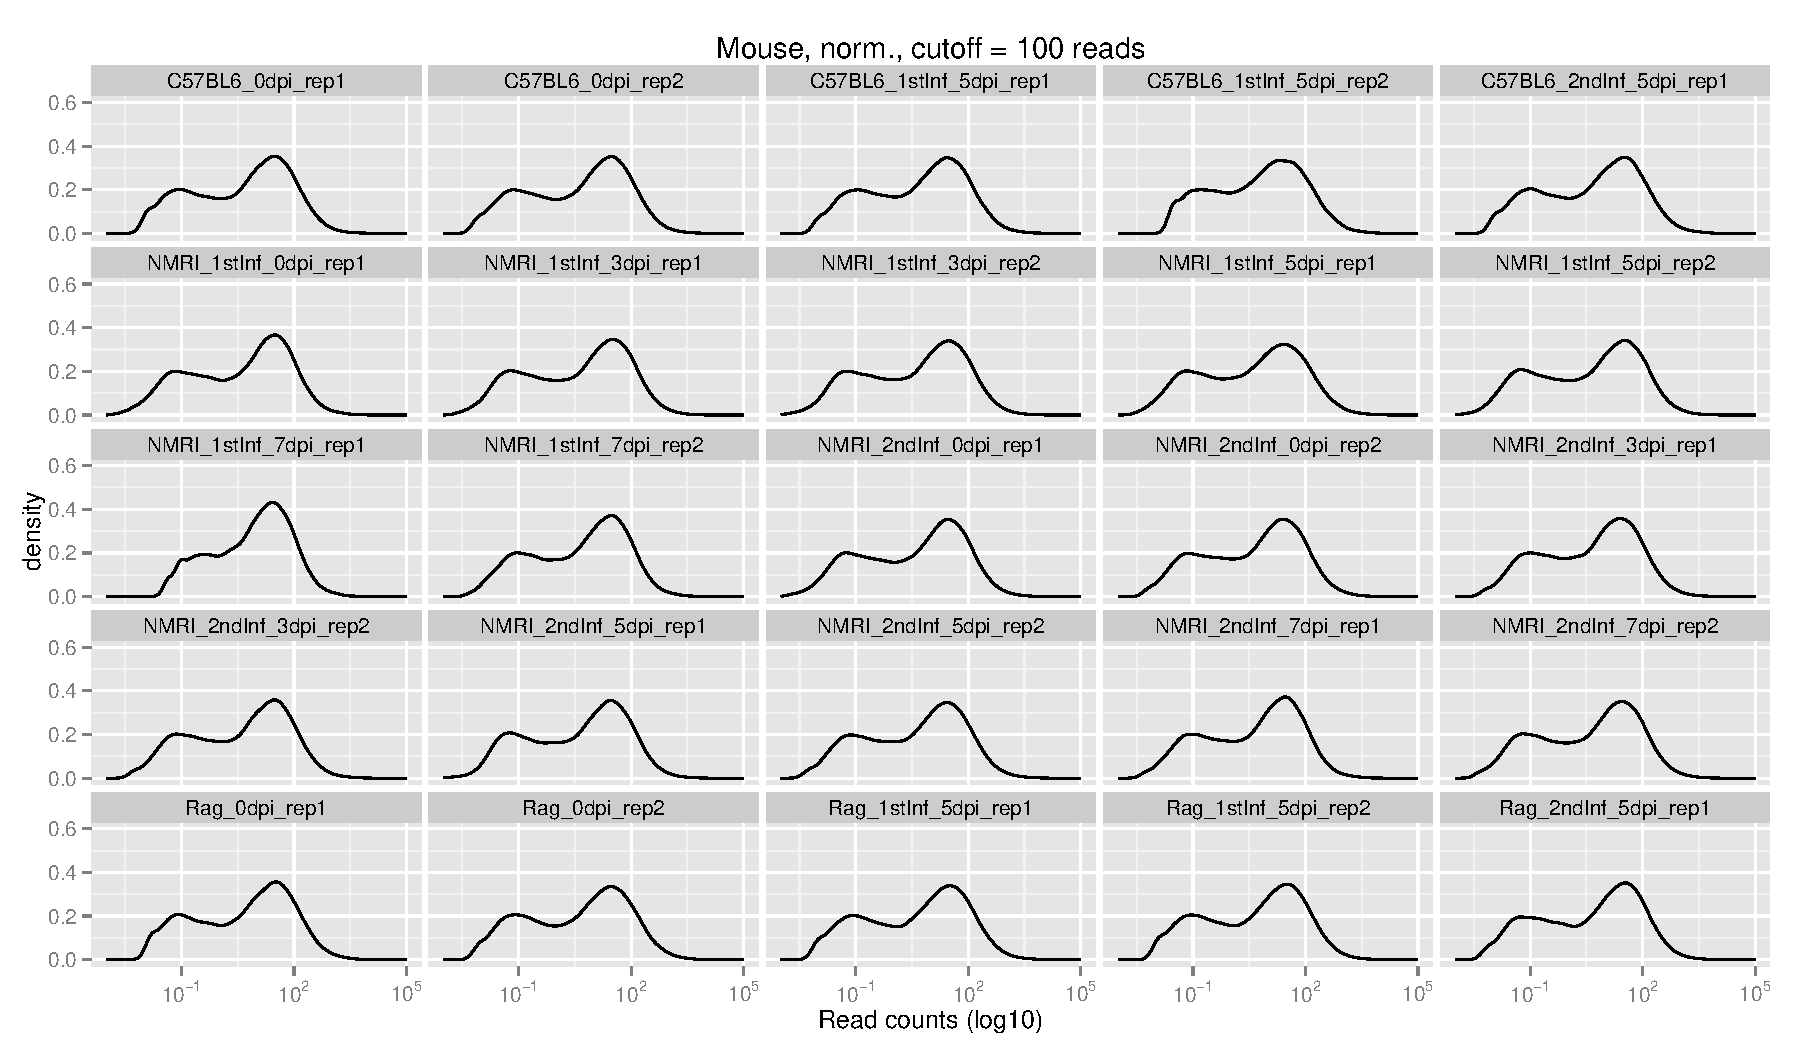
\includegraphics[width=0.8\textwidth]{distributions_normmouse100} % Include the image placeholder.png
\caption{Density distribution of normalised transcript counts (log10) for mouse samples with a cutoff of 100 (see Methods for details). All samples still have a bimodal distribution, however less pronounced compared to figures 1 and 2. The first density peak occurs at $<1$ transcripts as in Figure 2. The second density peak occurs at close to $10^2$ transcripts and did hence not change from the normalised data without cutoff (Figure 2).}
\end{center}
\end{figure}

% figure 4
\begin{figure}[h]
\begin{center}
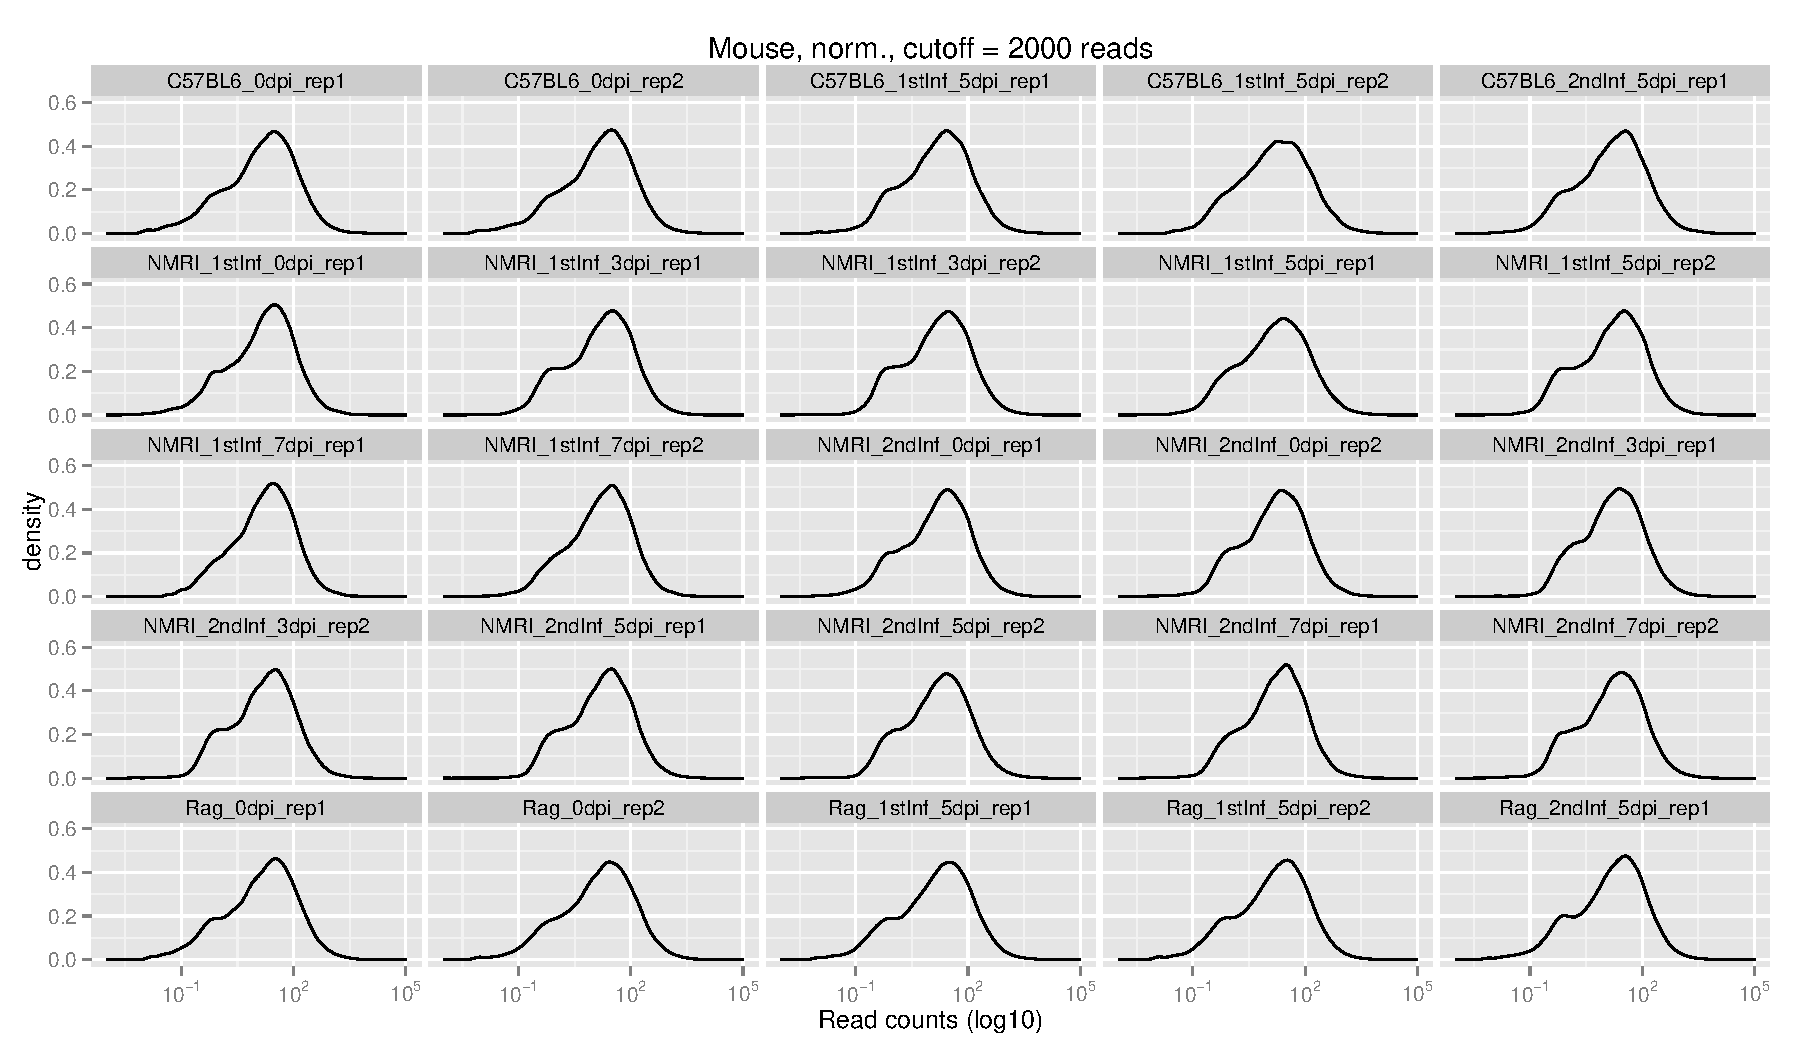
\includegraphics[width=0.8\textwidth]{distributions_normmouse2000} % Include the image placeholder.png
\caption{Density distribution of normalised transcript counts (log10) for mouse samples with a cutoff of 2000 (see Methods for details). The bimodality seen at lower cutoff values is strongly weakened or not detectable visually in some samples. It is however visually still seen in a majority of the samples. The first tendency to a density peak has shifted somewhat towards higher transcript counts (right) but is still $<1$ transcripts as in Figure 3. The second density peak occurs at close to $10^2$ transcripts and did hence not change from the normalised data with a lower cutoff (Figure 3).}
\end{center}
\end{figure}

% figure 5
\begin{figure}[h]
\begin{center}
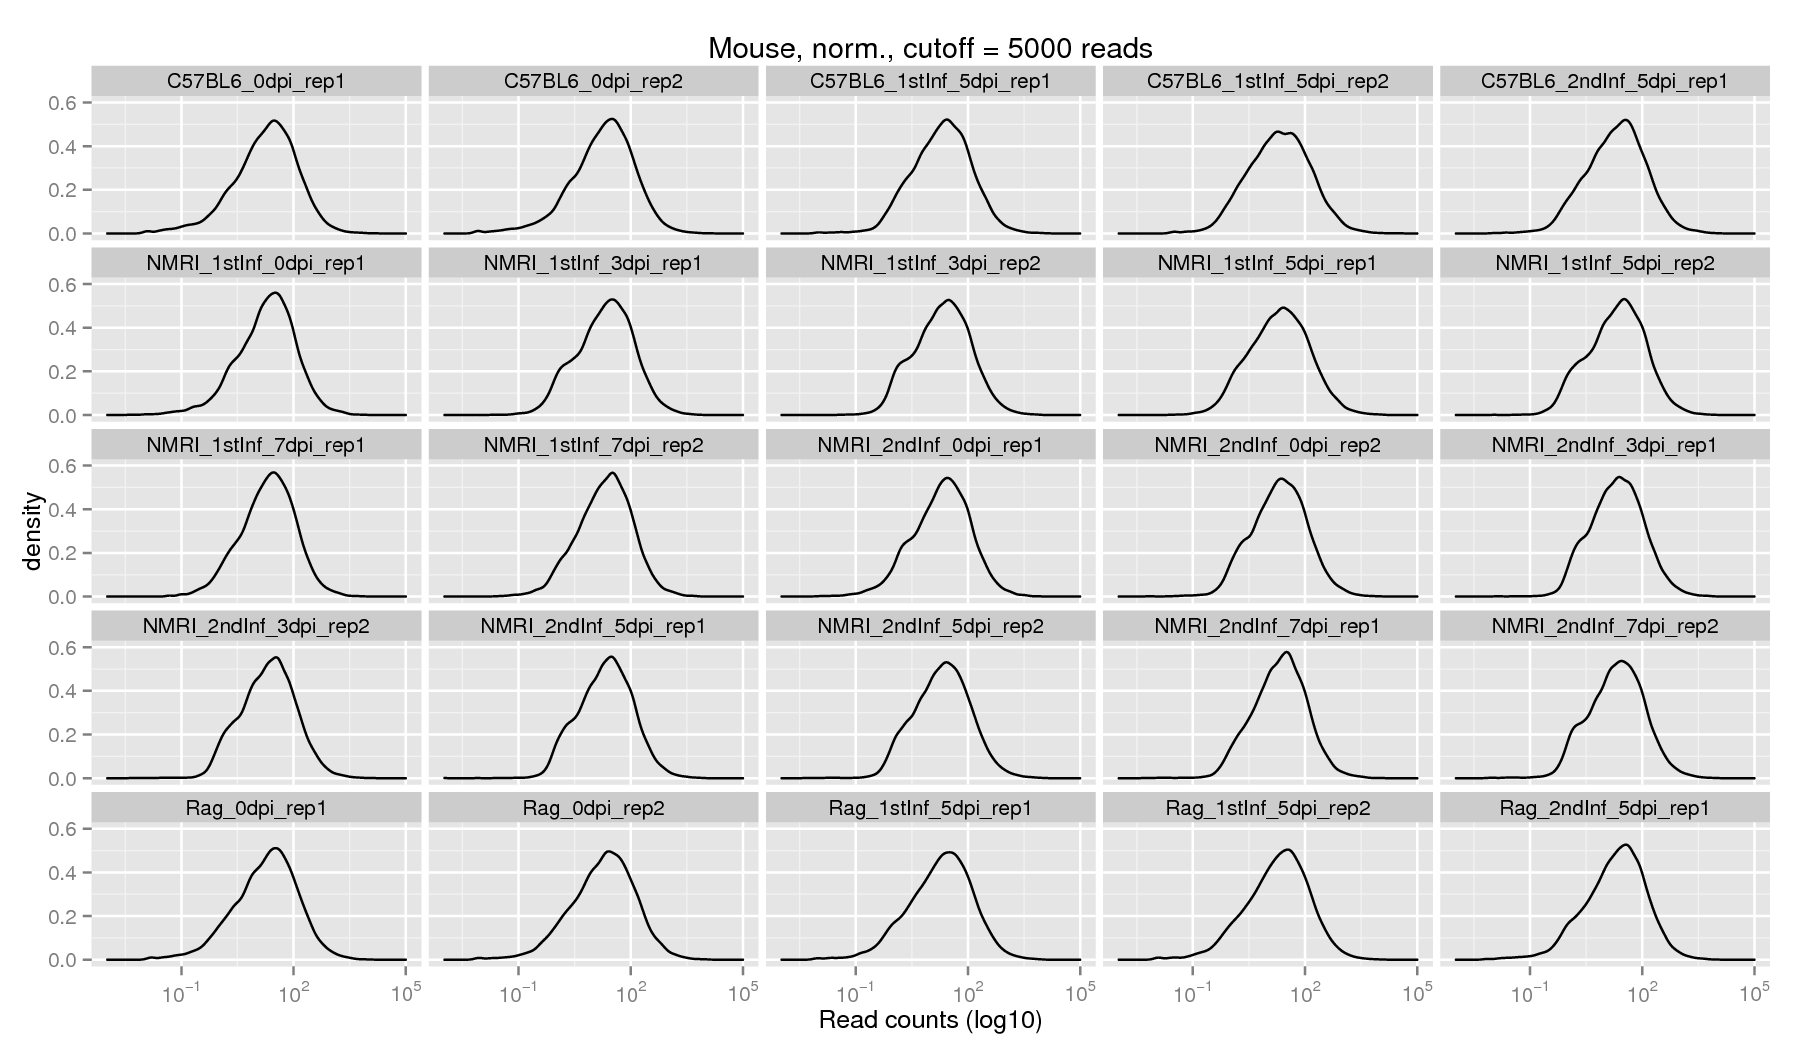
\includegraphics[width=0.8\textwidth]{distributions_normmouse5000} % Include the image placeholder.png
\caption{Density distribution of normalised transcript counts (log10) for mouse samples with a cutoff of 5000 (see Methods for details). The bimodality is not visually detectable in most samples, however it is still seen in \textit{e.g.} samples NMRI\_1stInf\_3dpi\_rep1 and NMRI\_2ndInf\_7dpi\_rep2. The major density peak remains at a value close to $10^2$ as in all the analysed normalised datasets (\textit{e.g.} Figure 2 or 4).}
\end{center}
\end{figure}

% figure 6
\begin{figure}[h]
\begin{center}
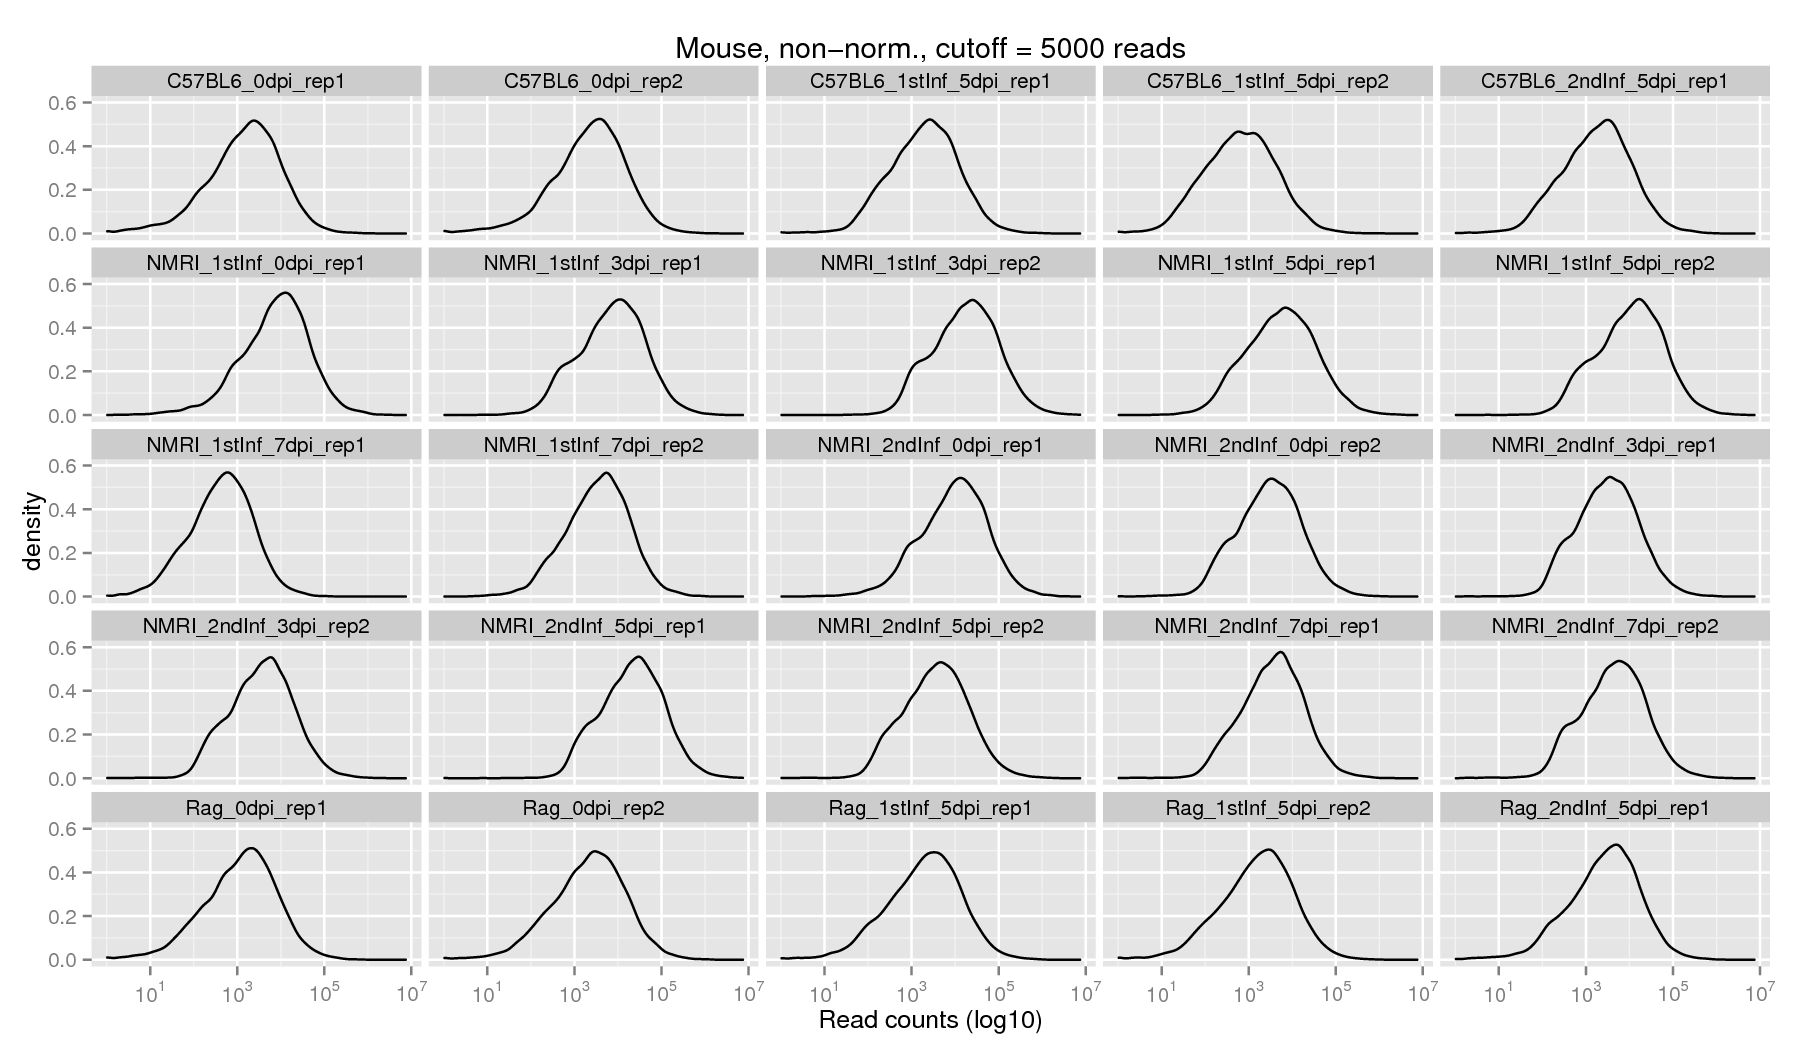
\includegraphics[width=0.8\textwidth]{distributions_mouse5000} % Include the image placeholder.png
\caption{Density distribution of raw transcript counts (log10) for mouse samples with a cutoff of 5000 (see Methods for details). The bimodality is not visually detectable in most samples, however it is still seen in \textit{e.g.} samples NMRI\_1stInf\_3dpi\_rep2 and NMRI\_2ndInf\_7dpi\_rep2. The major density peak is seen at a value over $10^2$, shifting it almost one order of magnitude compared to the normalised data with the same cutoff (Figure 5).}
\end{center}
\end{figure}

% figure 7
\begin{figure}[h]
\begin{center}
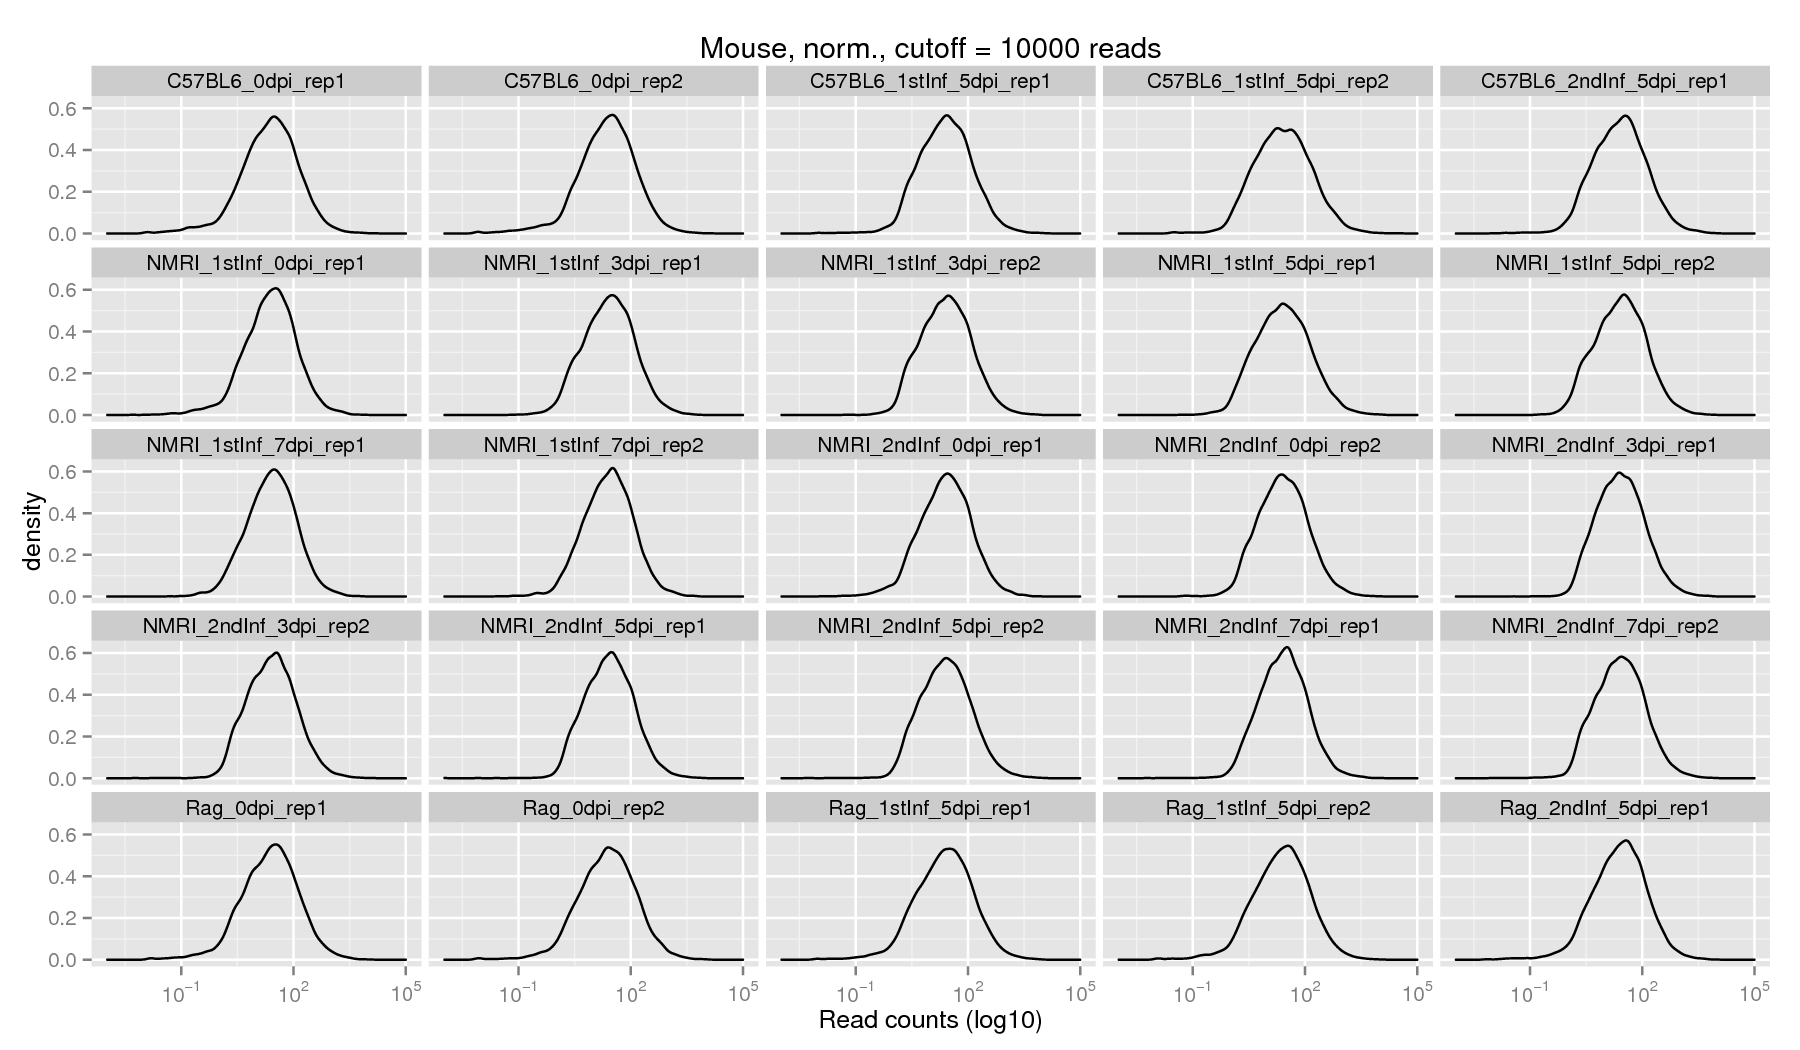
\includegraphics[width=0.8\textwidth]{distributions_normmouse10000} % Include the image placeholder.png
\caption{Density distribution of normalised transcript counts (log10) for mouse samples with a cutoff of 10000 (see Methods for details). The bimodality is not visually detectable in any sample apart from a minor indication in sample NMRI\_1stInf\_5dpi\_rep2. The major density peak remains at a value close to $10^2$ as in all the analysed normalised datasets (\textit{e.g.} Figure 2 or 4).}
\end{center}
\end{figure}


%----------------------------------------------------------------------------------------
%	SECTION 2 PARASITE DATA
%----------------------------------------------------------------------------------------

\section{Results for parasite}

% figure 8 
\begin{figure}[h]
\begin{center}
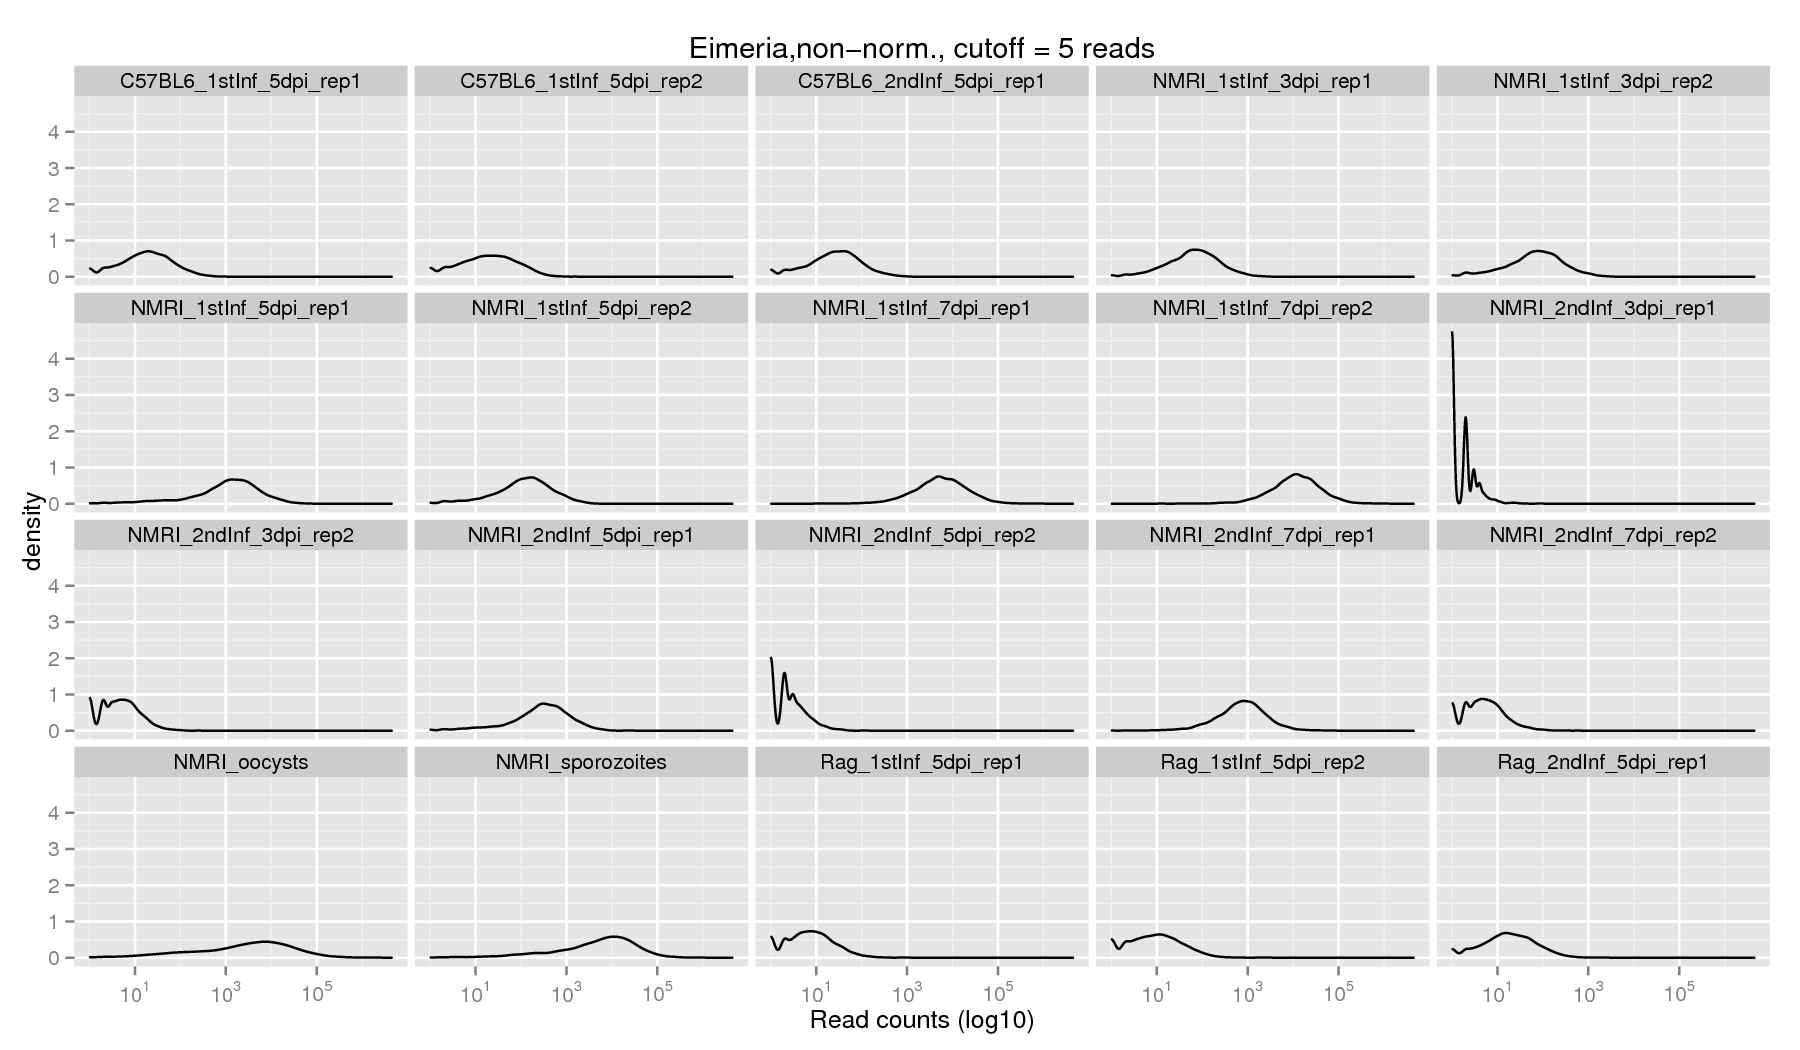
\includegraphics[width=0.8\textwidth]{distributions_Ef5} % Include the image placeholder.png
\caption{Density distribution of raw transcript counts (log10) for parasite samples with a cutoff of 5 (see Methods for details). Upon visual inspection distributions in most samples appear smooth and not contradictory to a negative binomial distribution. Density peak positions with regards to transcript counts (x-axis) are however at different orders of magnitudes between samples. Samples NMRI\_2ndInf\_3dpi\_rep1, NMRI\_2ndInf\_3dpi\_rep2, NMRI\_2ndInf\_5dpi\_rep2 and NMRI\_2ndInf\_7dpi\_rep2, however, do not.}
\end{center}
\end{figure}

% figure 9
\begin{figure}[h]
\begin{center}
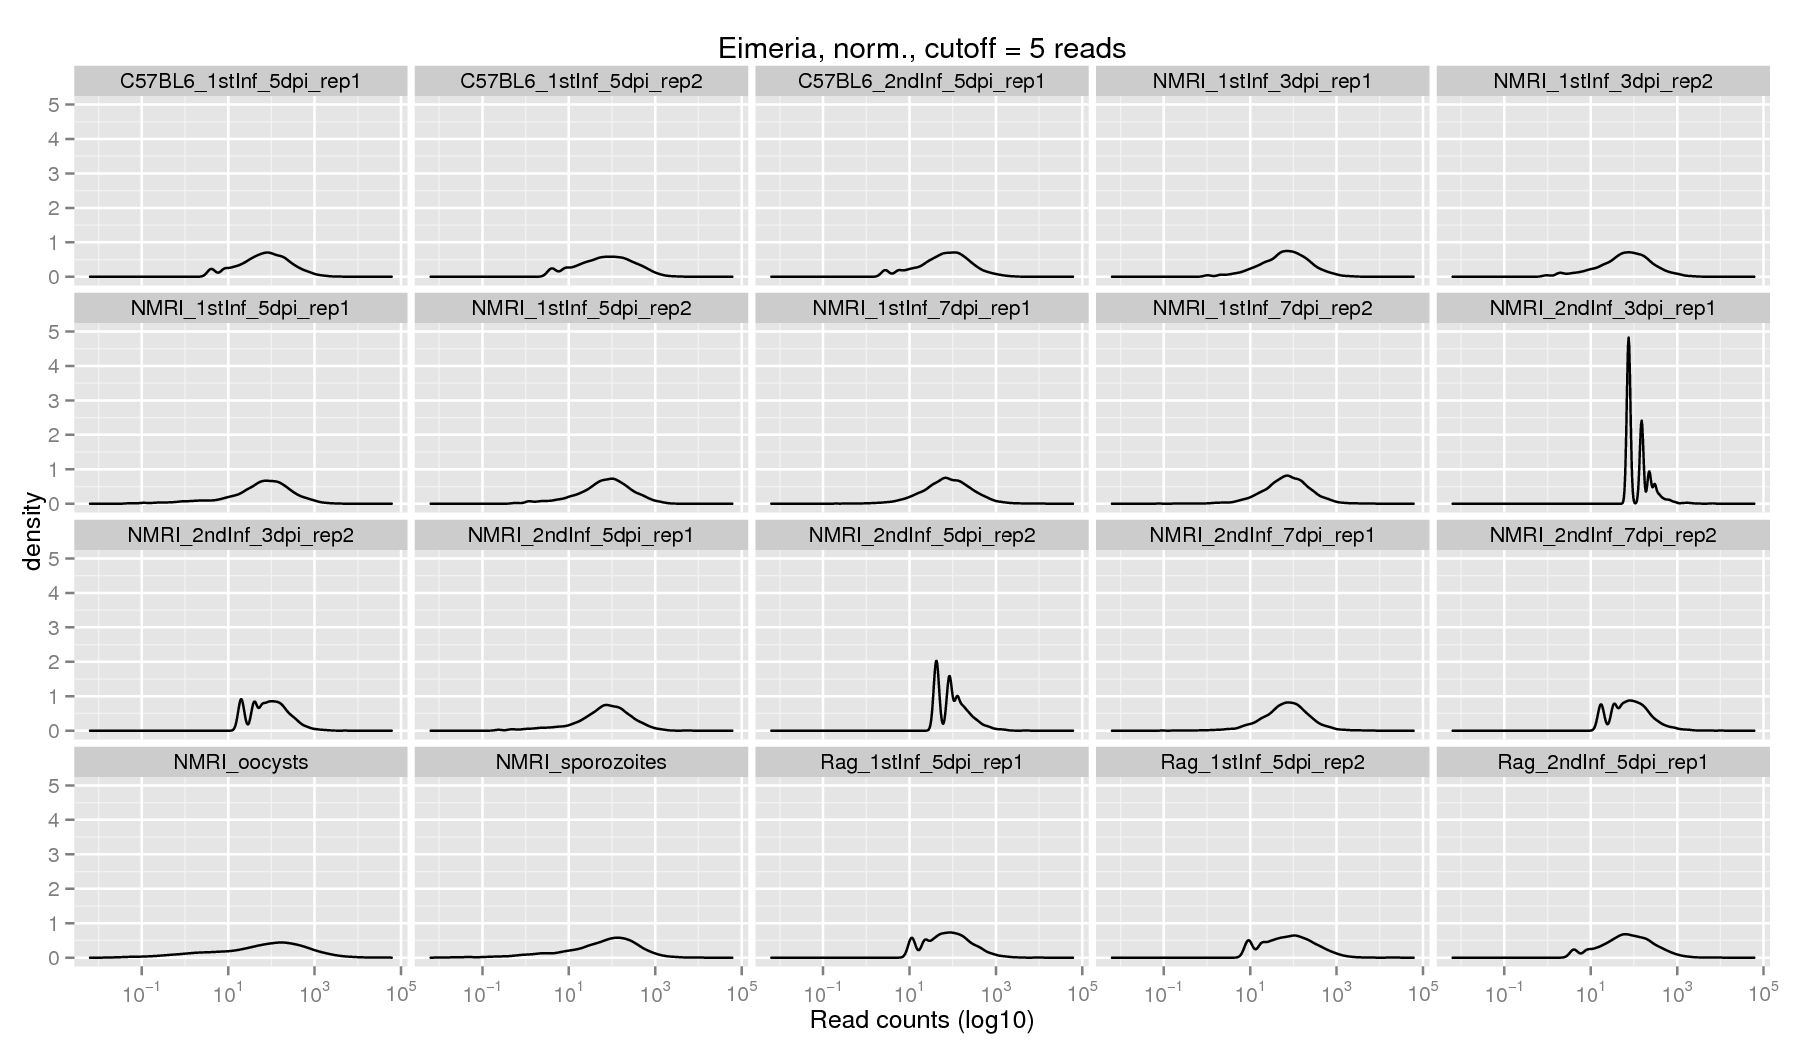
\includegraphics[width=0.8\textwidth]{distributions_Efnorm5} % Include the image placeholder.png
\caption{Density distribution of normalised transcript counts (log10) for parasite samples with a cutoff of 5 (see Methods for details). Upon visual inspection distributions in most samples appear smooth also in the normalised data. Density peaks are also in the same order of magnitude with regards to transcript counts (x-axis). Non-negative binomial samples in Figure 8 (NMRI\_2ndInf\_3dpi\_rep1, NMRI\_2ndInf\_3dpi\_rep2, NMRI\_2ndInf\_5dpi\_rep2 and NMRI\_2ndInf\_7dpi\_rep2) have more pronounced spikes in this normalised data. Additionally, samples Rag\_1stInf\_5dpi\_rep1 and Rag\_1stInf\_5dpi\_rep2 also have one additional peak in the lower range of the distribution, as do some other samples, but less pronounced.}
\end{center}
\end{figure}

% figure 10
\begin{figure}[h]
\begin{center}
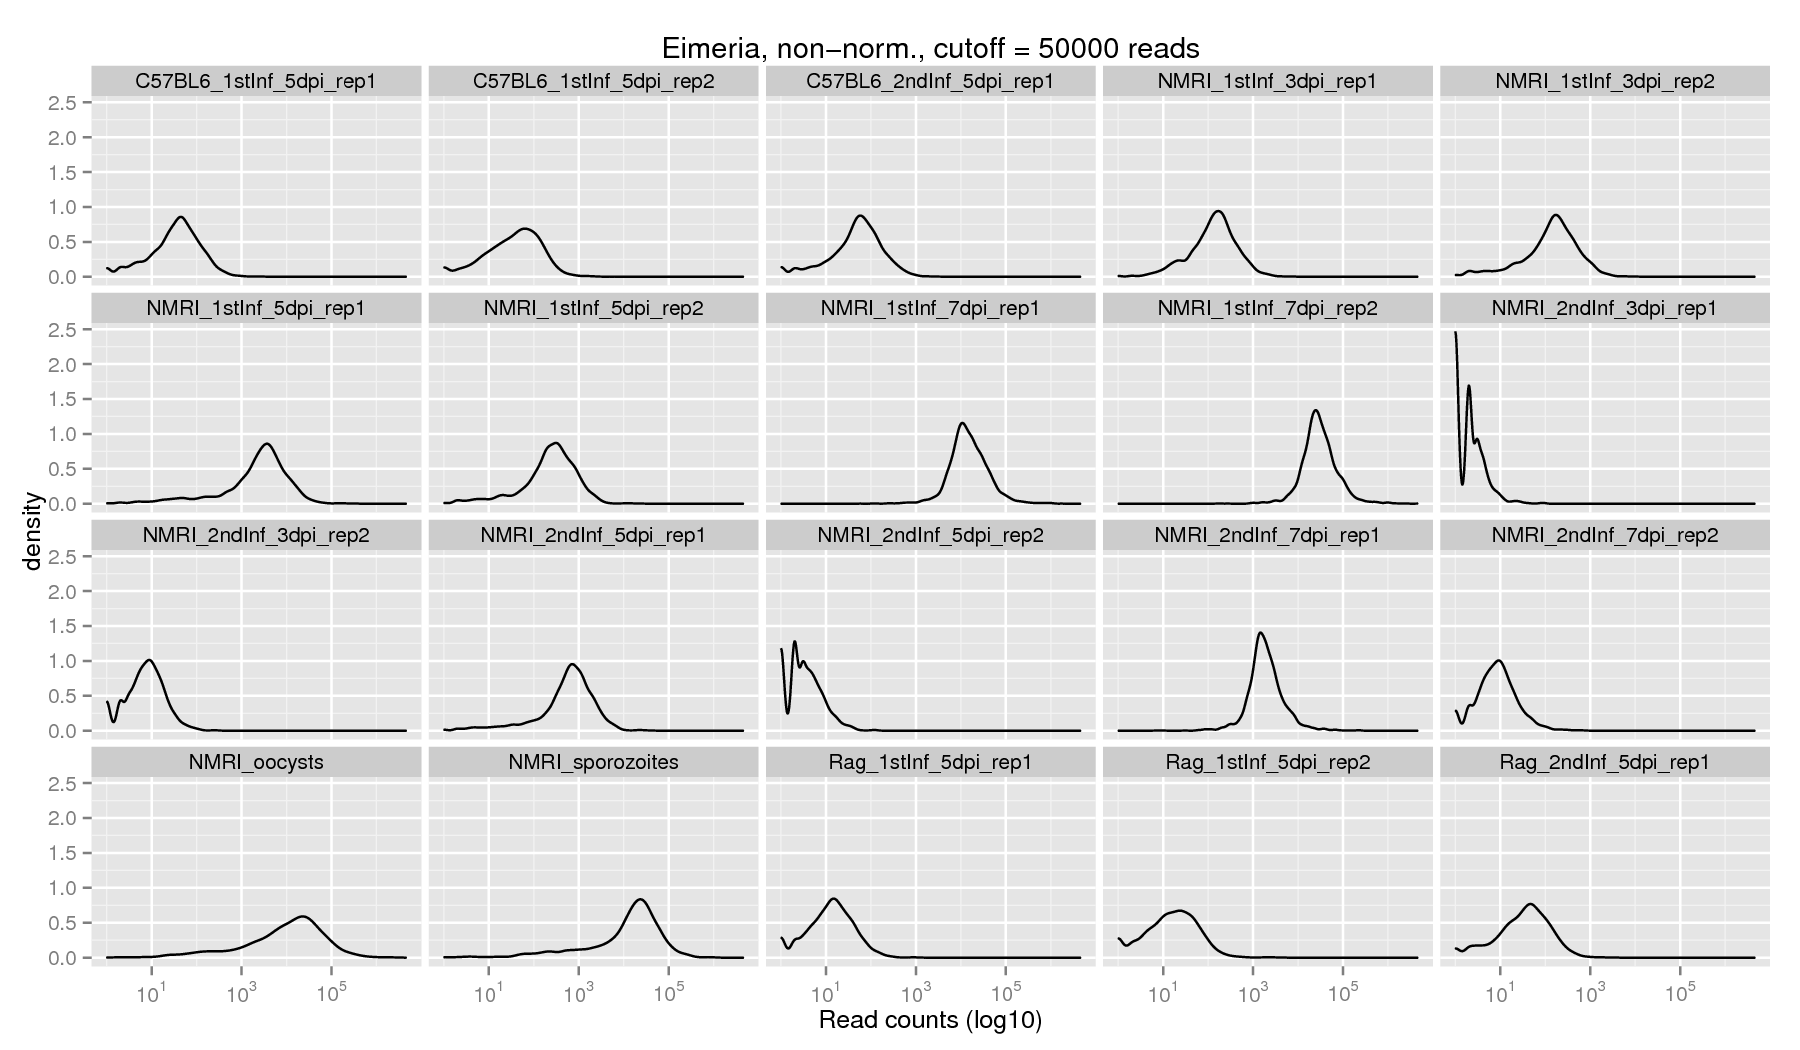
\includegraphics[width=0.8\textwidth]{distributions_Ef50000} % Include the image placeholder.png
\caption{Density distribution of raw transcript counts (log10) for parasite samples with a cutoff of 50000 (see Methods for details). Upon visual inspection distributions in most samples appear smooth. Non-negative binomial samples in Figure 8 and 9 (NMRI\_2ndInf\_3dpi\_rep1, NMRI\_2ndInf\_3dpi\_rep2, NMRI\_2ndInf\_5dpi\_rep2 and NMRI\_2ndInf\_7dpi\_rep2 have more than one density peak also when lowly expressed genes are removed with a high threshold (50000). Samples Rag\_1stInf\_5dpi\_rep1 and Rag\_1stInf\_5dpi\_rep2, however, seem smoother with only one density peak with this threshold.}
\end{center}
\end{figure}

% figure 11
\begin{figure}[h]
\begin{center}
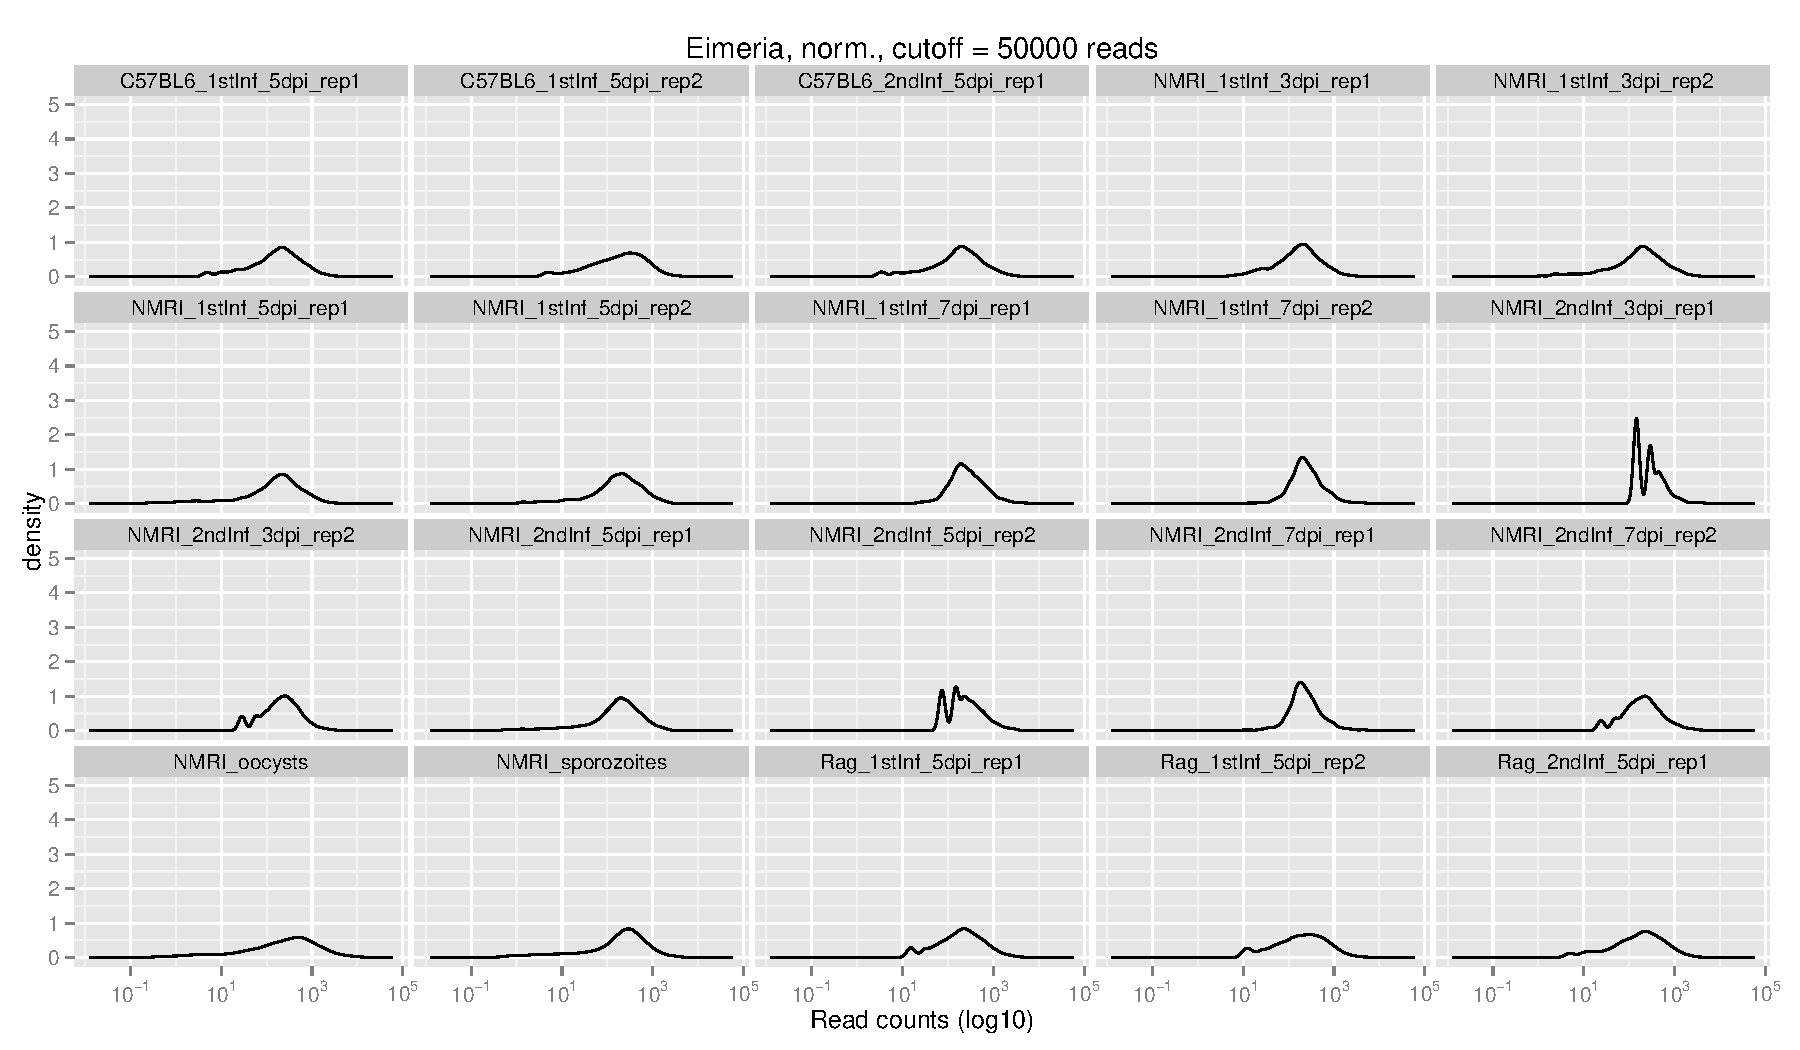
\includegraphics[width=0.8\textwidth]{distributions_Efnorm50000} % Include the image placeholder.png
\caption{Density distribution of normalised transcript counts (log10) for parasite samples with a cutoff of 50000 (see Methods for details). Upon visual inspection distributions in most samples appear smooth. Non-negative binomial samples are pronounced bimodal in this normalised data (NMRI\_2ndInf\_3dpi\_rep1, NMRI\_2ndInf\_3dpi\_rep2, NMRI\_2ndInf\_5dpi\_rep2 and NMRI\_2ndInf\_7dpi\_rep2). Samples Rag\_1stInf\_5dpi\_rep1 and Rag\_1stInf\_5dpi\_rep2 are also bimodal, however less pronounced.}
\end{center}
\end{figure}


%----------------------------------------------------------------------------------------
%	SECTION 5
%----------------------------------------------------------------------------------------

\section{Conclusions}

Mouse\\
The assumption of a negative binomial distribution underlies most differential gene expression analyses available. Similar bimodal expression patterns as in our mouse dataset have been reported (\textit{e.g.} ....) and suggested to be a result of a group of non-coding RNAs being sequenced. Since we are not interested in such RNA species in this project, different cutoff values were tested to find the lowest possible threshold for removing transcripts and gain a negative binomial distribution. By visual inspection (again: should we formalise/quantify this somehow?) we chose 5000 as the cutoff for further analysis.  \\

Parasite\\
The parasite data follows the expected distribution in most samples (although we have not formally tested it - check mean-var relationship to do that?). Bimodal or multipeak samples do not show unimodal distributions even with high cutoffs, \textit{i.e.} many transcripts required to map to one gene for the reads to be included. The four most obvious spiky samples are also the samples with fewest reads sequenced overall, which can explain the uneven distribution (make table to refer to?). We will exclude these four samples (NMRI\_2ndInf\_3dpi\_rep1, NMRI\_2ndInf\_3dpi\_rep2, NMRI\_2ndInf\_5dpi\_rep2 and NMRI\_2ndInf\_7dpi\_rep2) from all further analysis. It is not clear why there is such low coverage in these samples. Possibilities include poor infection success because of too low oocyst injection, mouse resistance due to \textit{e.g.} unknown previous infections or other unknown variability in the experiment. Because of this insecurity, these samples are also exculded from the mouse data. \\

The fact that the density peak occurs at similar read counts after normalisation in mouse and parasite data (respectively) is encouraging and indicates that normalisation is successful in both datasets. 


%----------------------------------------------------------------------------------------
%	SECTION 6
%----------------------------------------------------------------------------------------

%\section{Answers to Definitions}

%\begin{enumerate}
%\begin{item}
%The \emph{atomic weight of an element} is the relative weight of one of its atoms compared to C-12 with a weight of 12.0000000$\ldots$, hydrogen with a weight of 1.008, to oxygen with a weight of 16.00. Atomic weight is also the average weight of all the atoms of that element as they occur in nature.
%\end{item}
%\begin{item}
%The \emph{units of atomic weight} are two-fold, with an identical numerical value. They are g/mole of atoms (or just g/mol) or amu/atom.
%\end{item}
%\begin{item}
%\emph{Percentage discrepancy} between an accepted (literature) value and an experimental value is
%\begin{equation*}
%\frac{\mathrm{experimental\;result} - \mathrm{accepted\;result}}{\mathrm{accepted\;result}}
%\end{equation*}
%\end{item}
%\end{enumerate}

%----------------------------------------------------------------------------------------
%	BIBLIOGRAPHY
%----------------------------------------------------------------------------------------

%\bibliographystyle{apalike}

%\bibliography{sample}

%----------------------------------------------------------------------------------------


\end{document}
